\documentclass{article}
\usepackage[margin=0.8in]{geometry}
\usepackage{amsmath}
\usepackage{amssymb}
\usepackage{graphicx}
\usepackage{float}

\title{Mini-report for Programming Assignment 1: Question 4}
\author{Vishwak S \\
\texttt{CS15BTECH11043}}
\date{}

\begin{document}
\maketitle
\section*{Best Value for Hyperparameters for the \\
Gaussian and Polynomial kernels}
\begin{flushleft}
I conducted 50 experiments for finding a sub-optimal hyperparameter \(\sigma\) for the Gaussian Kernel and 10 experiments for finding a sub-optimal hyperparameter \(q\) for the Polynomial kernel. The experiments were performed using grid-search with \(q \in \{1, 2, \ldots, 10\}\) and \(\sigma \in \{0.1, 0.2, 0.3, \ldots, 5\}\). Below are the graphs of variation of train and validation accuracies with the hyperparameters for both kernels.

\begin{figure}[H]
\begin{minipage}{0.45\linewidth}
\centering
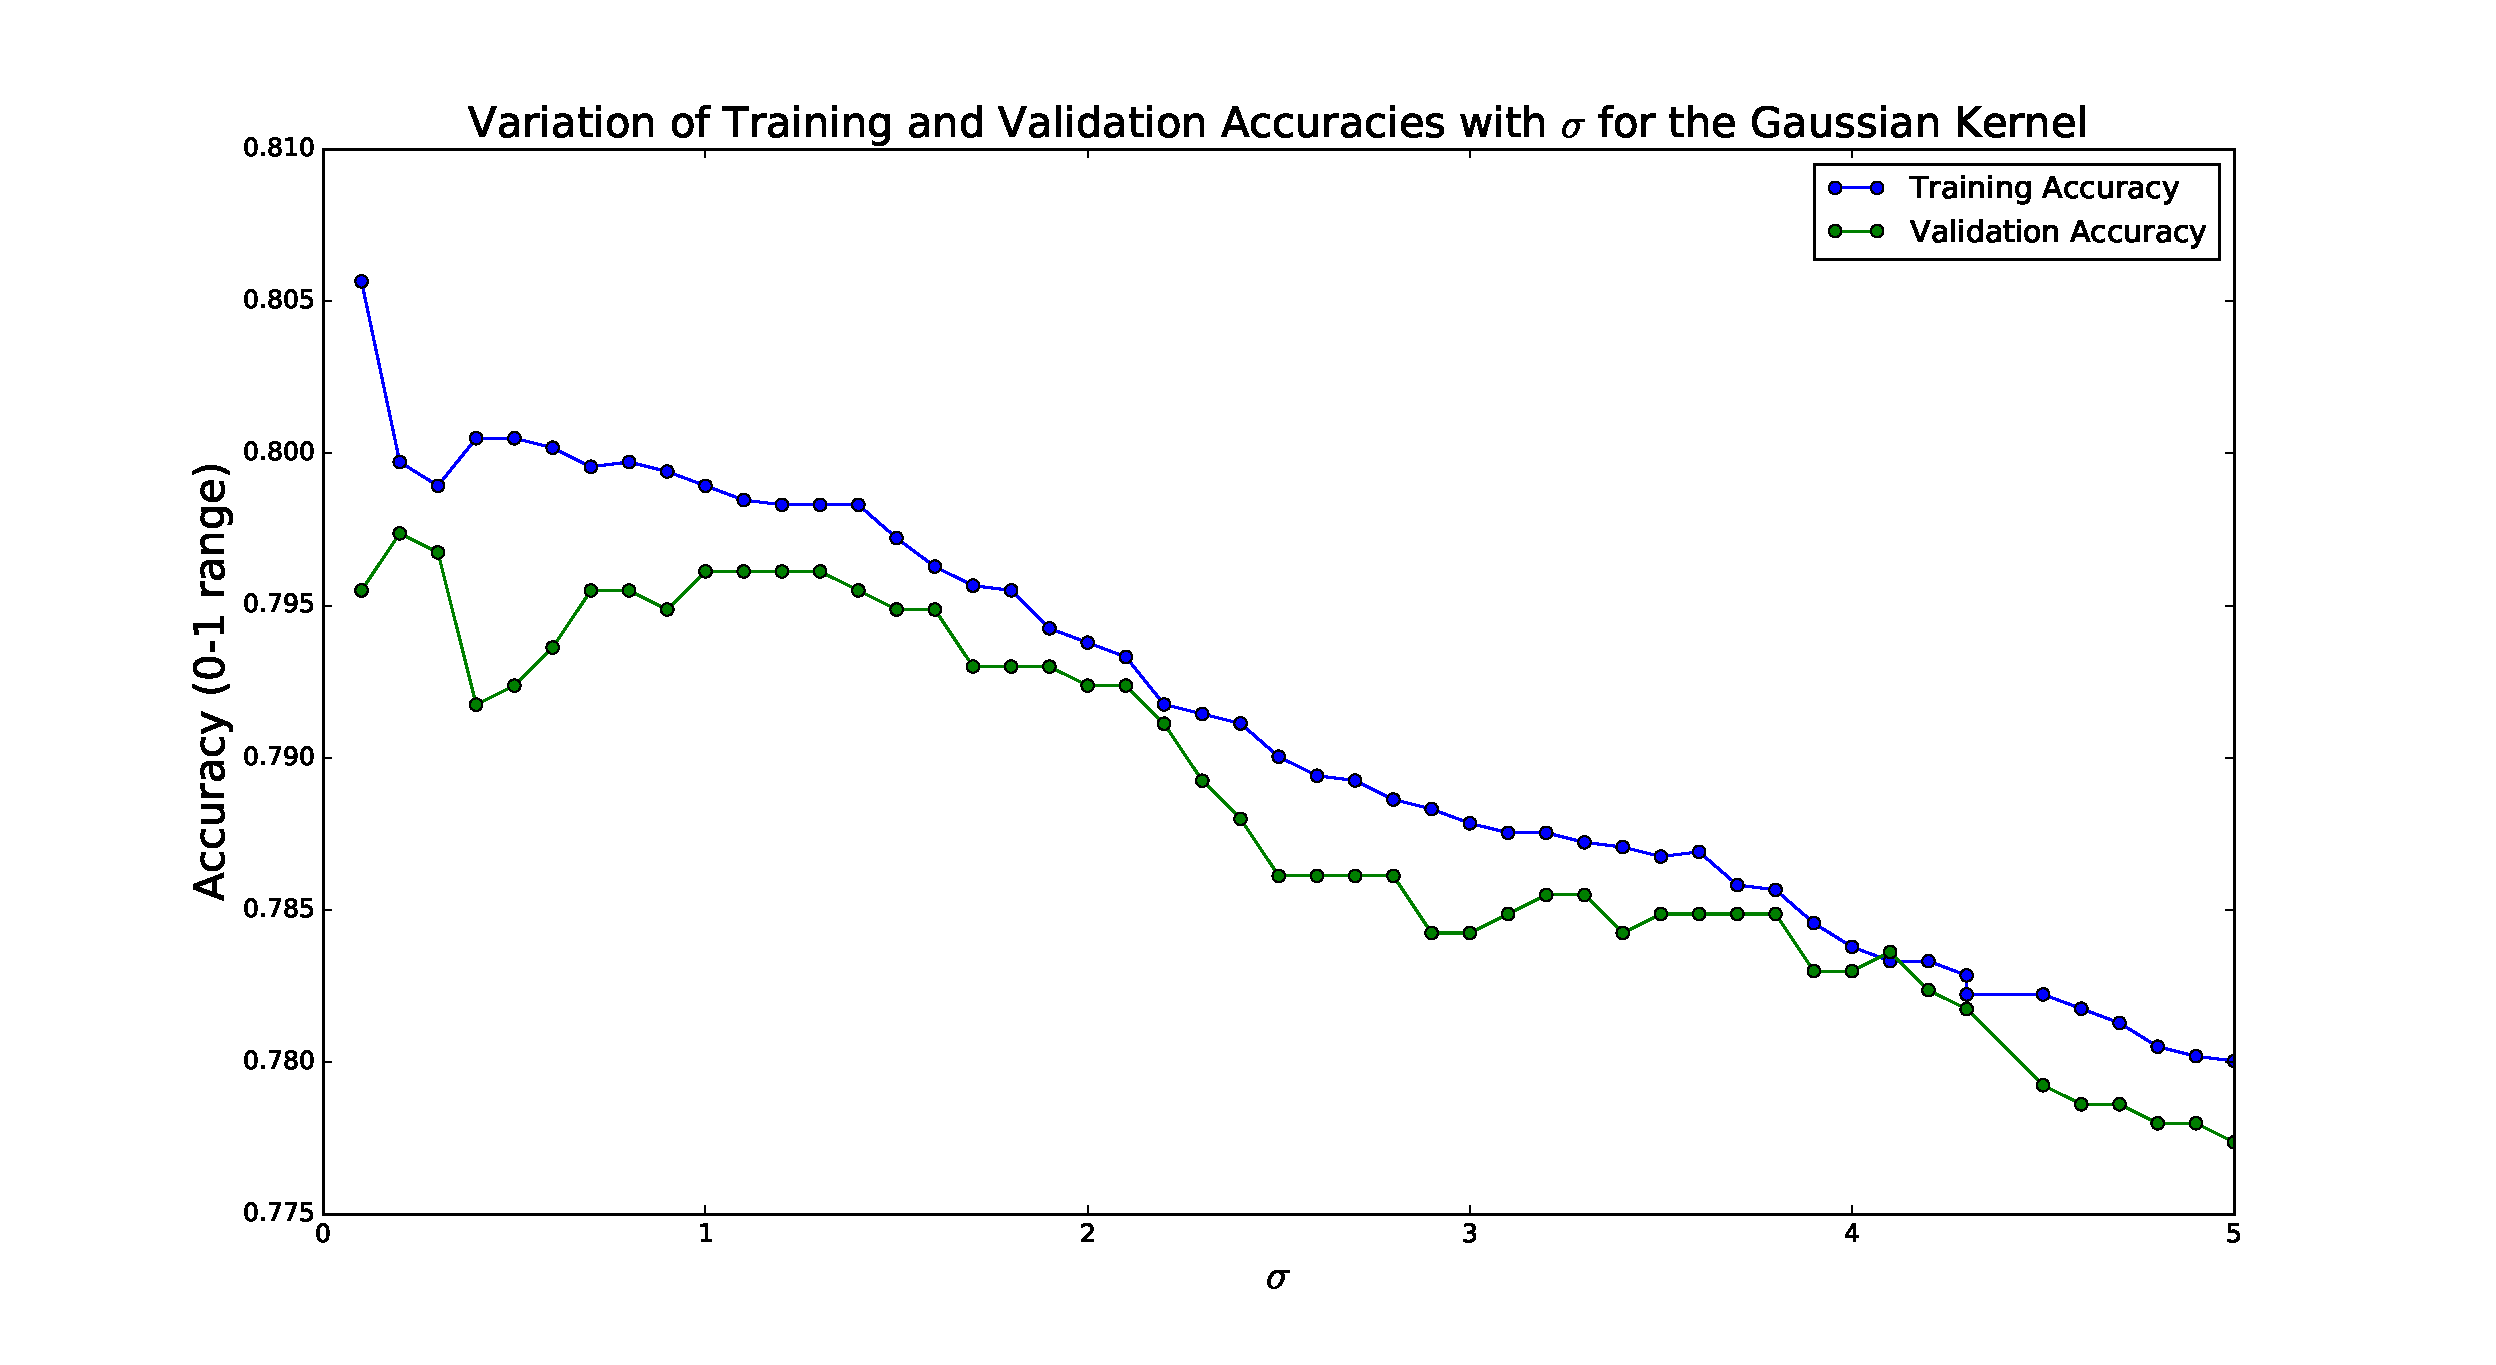
\includegraphics[width=0.95\textwidth]{./images/gaussian.eps}
\end{minipage}
\hfill
\begin{minipage}{0.45\linewidth}
\centering
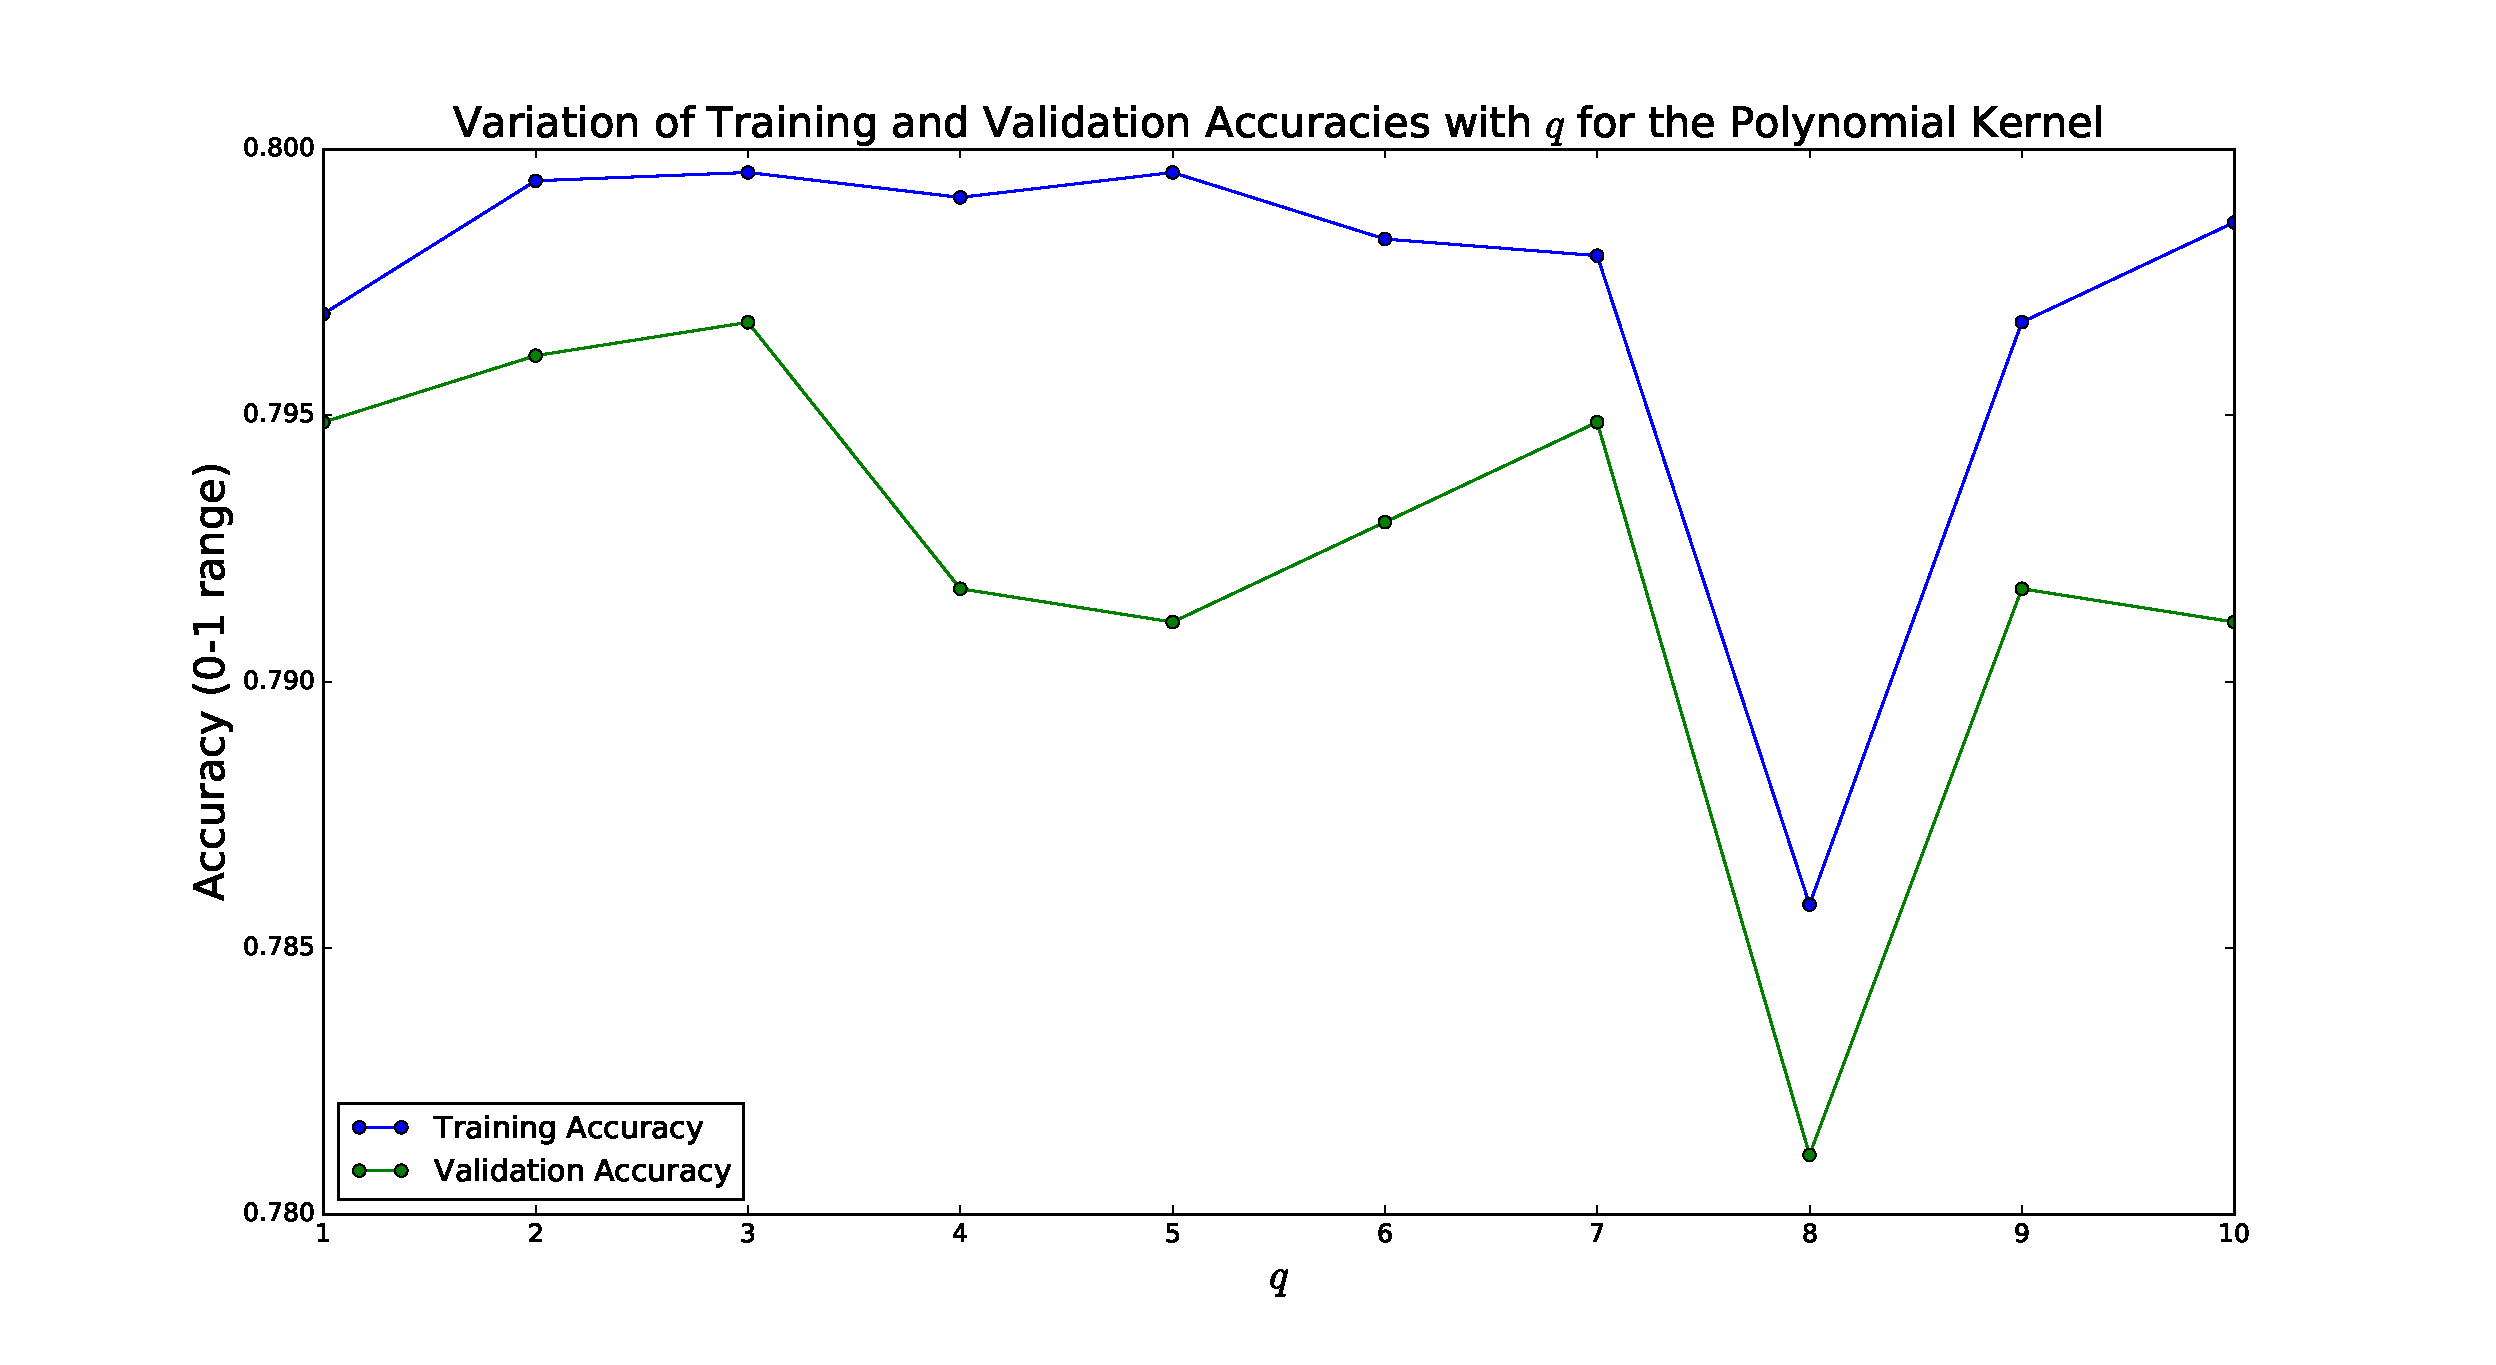
\includegraphics[width=0.95\textwidth]{./images/polynomial.eps}
\end{minipage}
\end{figure}

From this I chose, \(q_{\text{opt}} = 3\) and \(\sigma_{\text{opt}} = 0.2\). The Best Accuracies where compared alongside each other, and Gaussian kernel performed best. Below is a bar chart:
\begin{figure}[H]
\centering
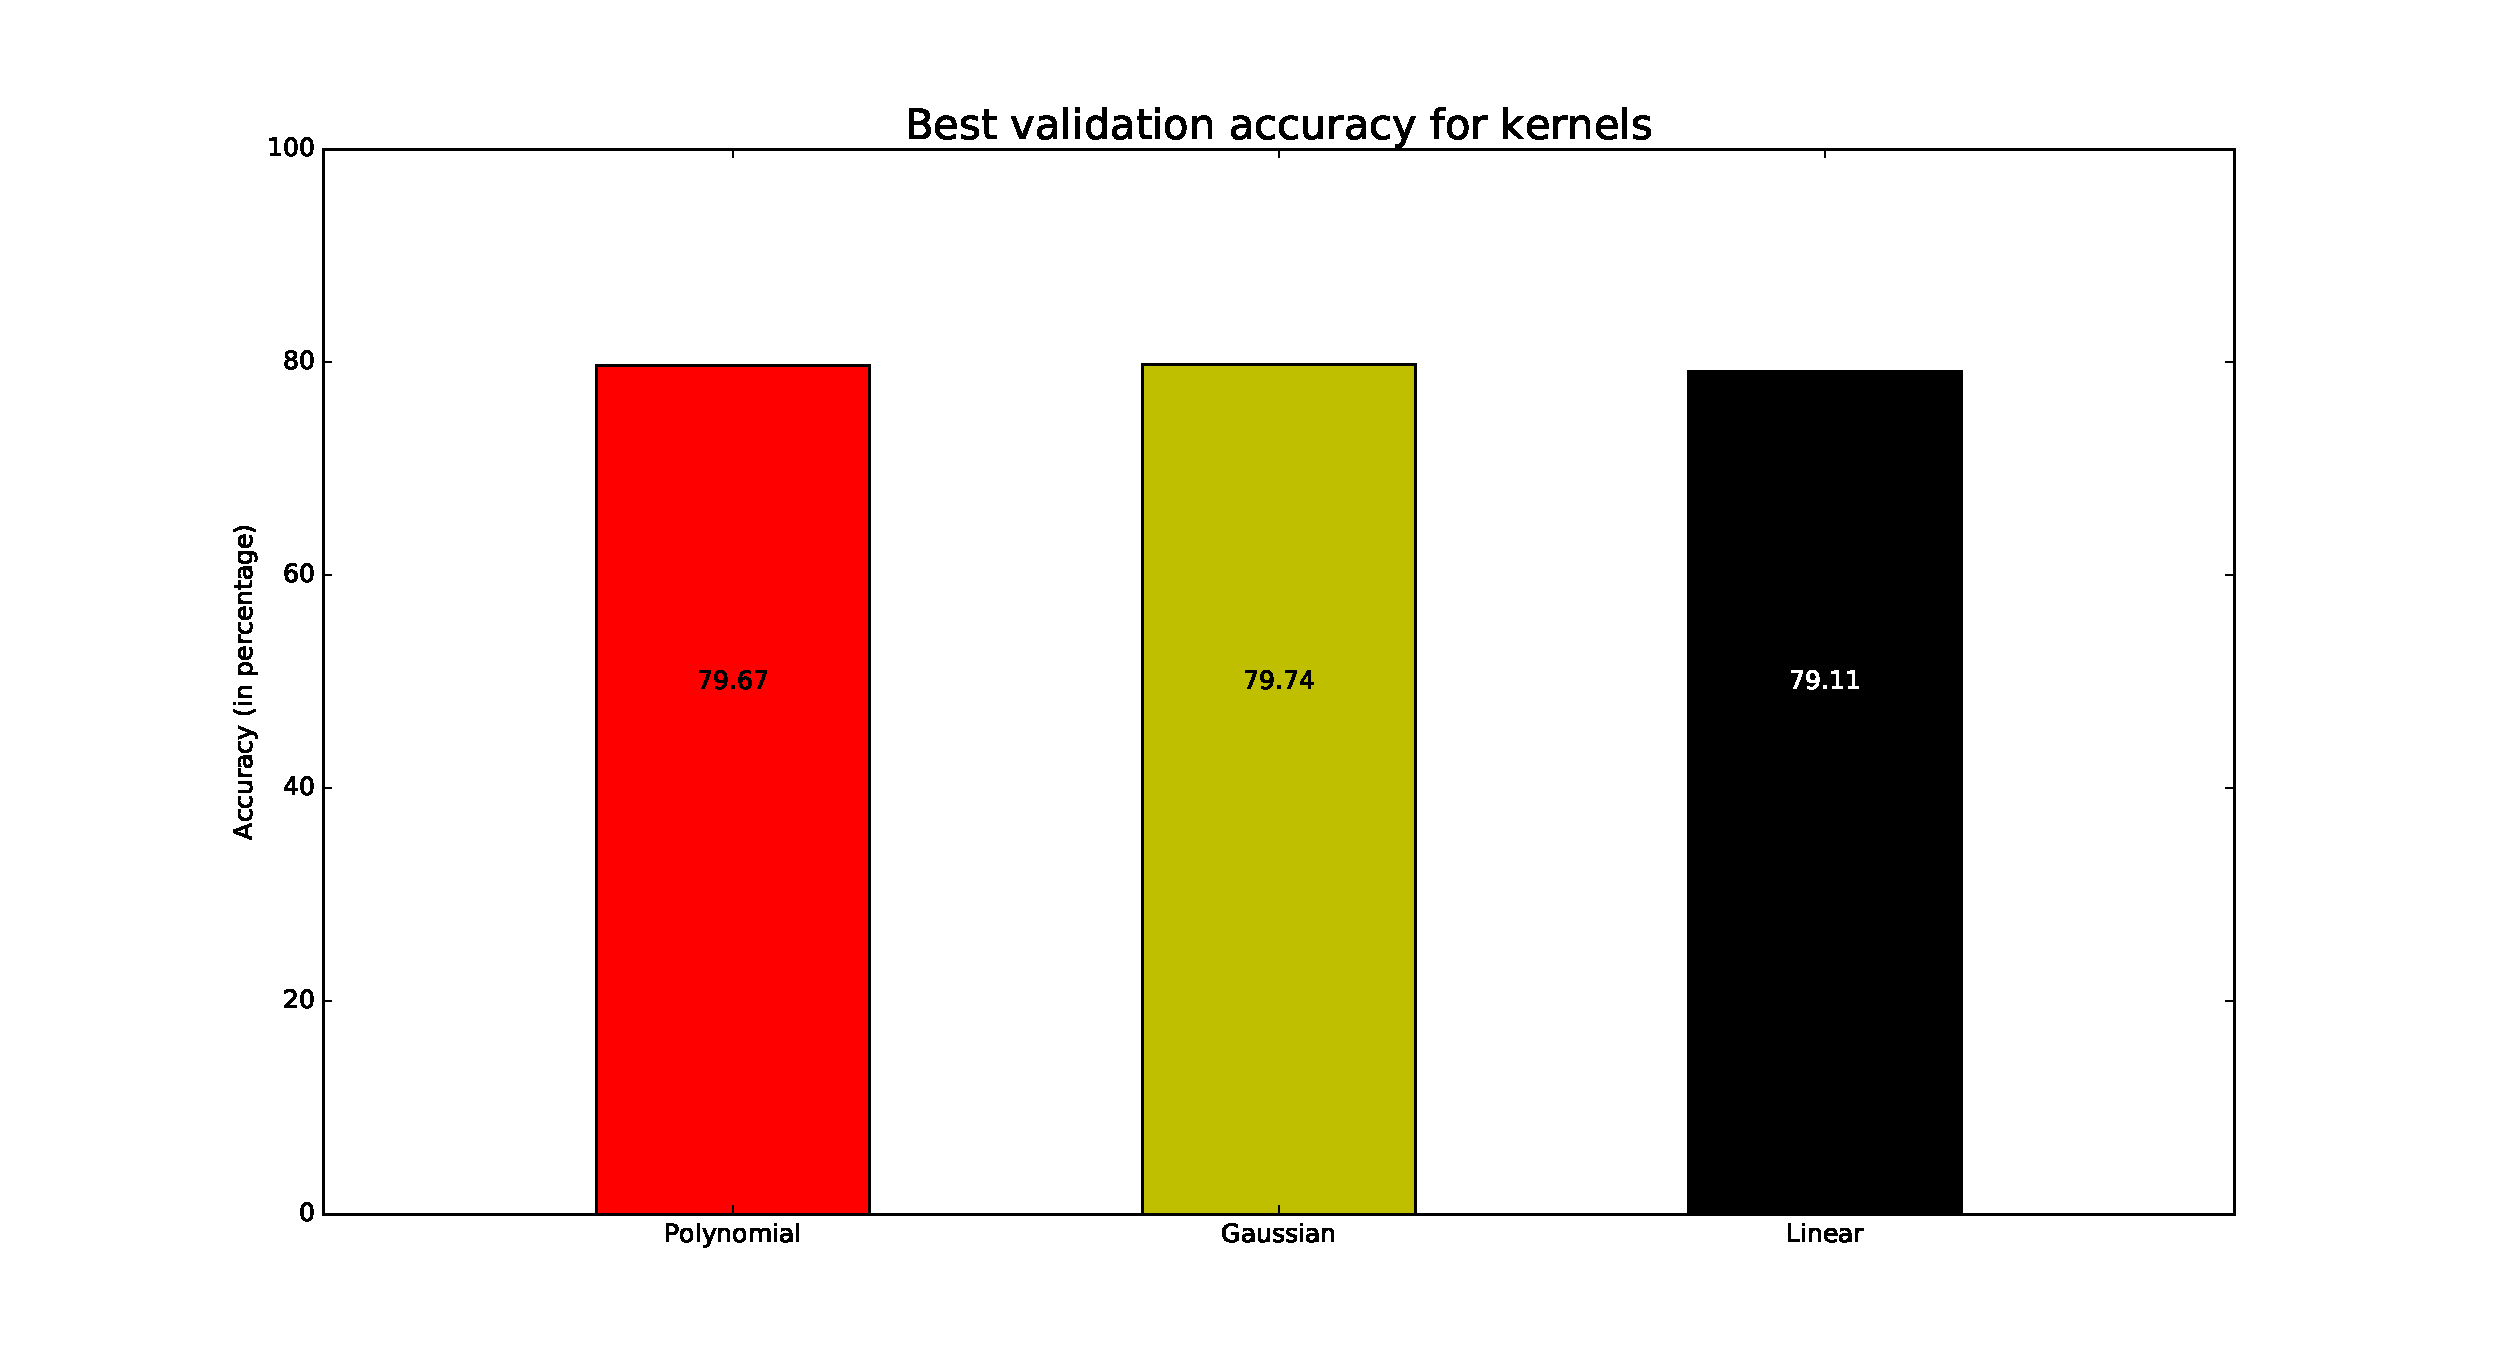
\includegraphics[width=0.75\linewidth]{./images/comparison_3.eps}
\end{figure}
\end{flushleft}
\end{document}
